\section{Methodology}
Here, we provide the full stack of programs and methods used to perform this experiment.

\subsection{Image Captioning}
For each image provided to our program, we first run it through the Dense Relational Captioning model. This provides us with a JSON filled with visual information about the image, as seen in Figure 1. Included in the data created are the captions for the relations between dense regions and the coordinates of the bounding boxes that representing the captured regions. We manually annotate this JSON with another field that assigns to of the bounding boxes to each generated caption as demonstrated in Figure 2. This completes the visual information needed to move onto the logic section of the program. 

\begin{figure}[htbp]
\centerline{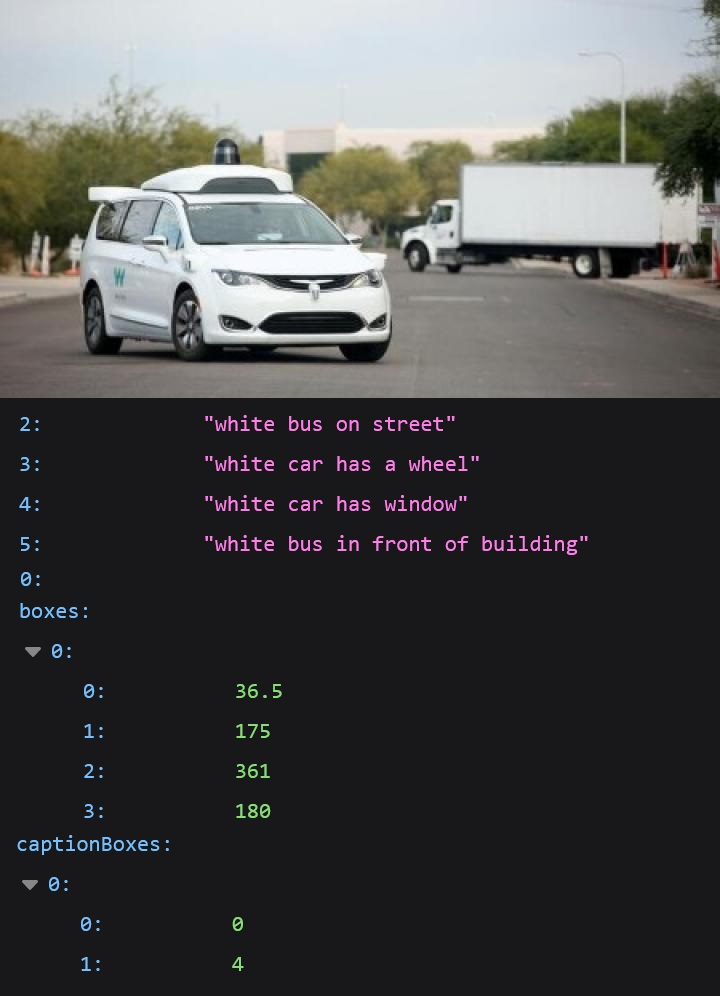
\includegraphics[width=.5\textwidth]{img1.jpg}}
\caption{A sample of the captions generated and one of the bounding boxes generated with Dense Relational Captioning model for the given image after manual annotation. The "boxes" section contains four numbers represent the X-position, Y-position, width, and height of the bounding box. The "captionBoxes" section states that the relation in caption zero is between region zero and region four. \protect\footnotemark[1]}
\label{fig1}
\end{figure}
\footnotetext[1]{Source of image: \url{https://www.reuters.com/business/autos-transportation/us-labor-leader-calls-human-drivers-automated-vehicles-2021-05-17/}.}

\subsection{Commonsense Reasoning}
The visual information provided by the image captioning earlier is converted into logic predicate form. A program is run that uses spacy\cite{spacy2} to parse each natural language caption into two objects and a relation. It then attaches the manually added bounding boxes to the relation. Finally, it creates a list of separate predicates that represent each of the boxes and their coordinate information. This information is used as the input for a main PROLOG program that contains our commonsense knowledge and reasoning. Four queries are made for each image:
\begin{itemize}
\item \begin{verbatim} select_action(brake, T)
\end{verbatim}
\item \begin{verbatim} select_action(change_lane_right, T)
\end{verbatim}
\item \begin{verbatim} select_action(change_lane_left, T)
\end{verbatim}
\item \begin{verbatim} select_action(go_forward, T)
\end{verbatim}
\end{itemize}
The program then returns a truth statement that represents whether or not each action is possible. 

The main goal for each logic statement is to detect if there is an object or entity that is actively obstructing each action. Unlike most autonomous vehicles, we are operating with only an image and no additional information. To determine if it is safe to take an action, we look at the objects at different regions of the picture. We use commonsense knowledge and reasoning to determine if the detected objects are something that we can drive on (e.g. roads or streets) or are otherwise obstructing our path. This is done for all actions except for braking. For a brake to be safe, we simply determine if there is something in our forward path and that it is expected of us to do so. 
